\documentclass{article}
\usepackage{tikz}
\usetikzlibrary{arrows}

\tikzset{
  treenode/.style = {align=center, inner sep=0pt, text centered,
    font=\sffamily},
  bt_l/.style = {treenode, rectangle, draw=black, fill=white,
    minimum width=0.5em, minimum height=0.5em}, 
  bt_n/.style = {treenode, rectangle, draw=black, fill=black,
    minimum width=0.5em, minimum height=0.5em}
}

\begin{document}

\begin{figure}[!htbp]
\centering

\begin{tikzpicture}[>=stealth',level/.style={sibling distance = 1cm/#1,
  level distance = 0.5cm}] 
\node [bt_l] {}
; 
\end{tikzpicture}

\vspace{0.5cm}

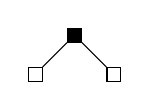
\begin{tikzpicture}[>=stealth',level/.style={sibling distance = 1cm/#1,
  level distance = 0.5cm}] 
\node [bt_n] {}
    child{ node [bt_l] {} } 
    child{ node [bt_l] {} }
; 
\end{tikzpicture}

\begin{minipage}{.15\textwidth}
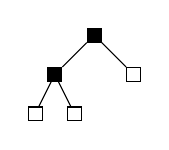
\begin{tikzpicture}[>=stealth',level/.style={sibling distance = 1cm/#1,
  level distance = 0.5cm}] 
\node [bt_n] {}
    child{ node [bt_n] {} 
	child{ node [bt_l] {}}
	child{ node [bt_l] {}}
	} 
    child{ node [bt_l] {} }
; 
\end{tikzpicture}
\end{minipage}
\begin{minipage}{.15\textwidth}
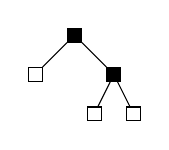
\begin{tikzpicture}[>=stealth',level/.style={sibling distance = 1cm/#1,
  level distance = 0.5cm}] 
\node [bt_n] {}
    child{ node [bt_l] {} }
    child{ node [bt_n] {} 
	child{ node [bt_l] {} }
	child{ node [bt_l] {} }
	} 
; 
\end{tikzpicture}
\end{minipage}

\begin{minipage}{.15\textwidth}
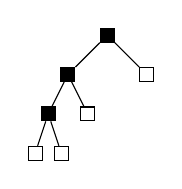
\begin{tikzpicture}[>=stealth',level/.style={sibling distance = 1cm/#1,
  level distance = 0.5cm}] 
\node [bt_n] {}
    child{ node [bt_n] {} 
	child{ node [bt_n] {}
		child { node [bt_l] {}}
		child { node [bt_l] {}}
	}
	child{ node [bt_l] {}}
	} 
    child{ node [bt_l] {} }
; 
\end{tikzpicture}
\end{minipage}
\begin{minipage}{.15\textwidth}
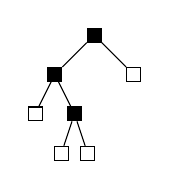
\begin{tikzpicture}[>=stealth',level/.style={sibling distance = 1cm/#1,
  level distance = 0.5cm}] 
\node [bt_n] {}
    child{ node [bt_n] {} 
	child{ node [bt_l] {}}
	child{ node [bt_n] {}
		child { node [bt_l] {}}
		child { node [bt_l] {}}
	}
	} 
    child{ node [bt_l] {} }
; 
\end{tikzpicture}
\end{minipage}
\begin{minipage}{.15\textwidth}
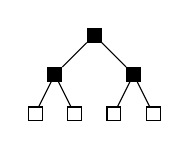
\begin{tikzpicture}[>=stealth',level/.style={sibling distance = 1cm/#1,
  level distance = 0.5cm}] 
\node [bt_n] {}
    child{ node [bt_n] {} 
	child { node [bt_l] {}}
	child { node [bt_l] {}}
	} 
    child{ node [bt_n] {} 
	child { node [bt_l] {}}
	child { node [bt_l] {}}
	}
; 
\end{tikzpicture}
\end{minipage}
\begin{minipage}{.15\textwidth}
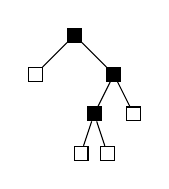
\begin{tikzpicture}[>=stealth',level/.style={sibling distance = 1cm/#1,
  level distance = 0.5cm}] 
\node [bt_n] {}
    child{ node [bt_l] {} }
    child{ node [bt_n] {} 
	child{ node [bt_n] {}
		child { node [bt_l] {}}
		child { node [bt_l] {}}
	}
	child{ node [bt_l] {}}
	} 
; 
\end{tikzpicture}
\end{minipage}

\caption{Number of binary trees for $n\in\{0,1,2,3\}$}\label{fig:catalan}
\end{figure}

\end{document}
